\emph{October, 2011}. Tom's day-job involves finding patterns in market
data (see
\href{http://www.ted.com/talks/kevin_slavin_how_algorithms_shape_our_world.html}{Kevin
Slavin's TED talk}). He reads philosophy and does some other programming
work in his spare time. However, he doesn't take the Occupy Wall Street
protest very seriously. But one of these evenings, one of the protestors
catches his attention. She's dressed rather strikingly. They talk, and
he comes away thinking about something she said:
``\emph{\href{http://www.nycga.net/files/2011/11/DeclarationFlowchart\_v2\_large.jpg}{All our grievances are interconnected}.}'' What if all the solutions are
interconnected too? Night time: Tom becomes increasingly obsessed with
this idea. He's pulling down lots of web pages from the internet ---
again, looking for patterns. What would it take for OWS folks to solve
the problems they worry so much about? He starts working on a tool
that's geared towards learning and sharing skills, while working on real
projects. At first, it's just hackers who are using the tool, but over
time they adapt it for popular use. Things start to get
interesting\ldots{} 

\begin{figure}[htbp]
\centering
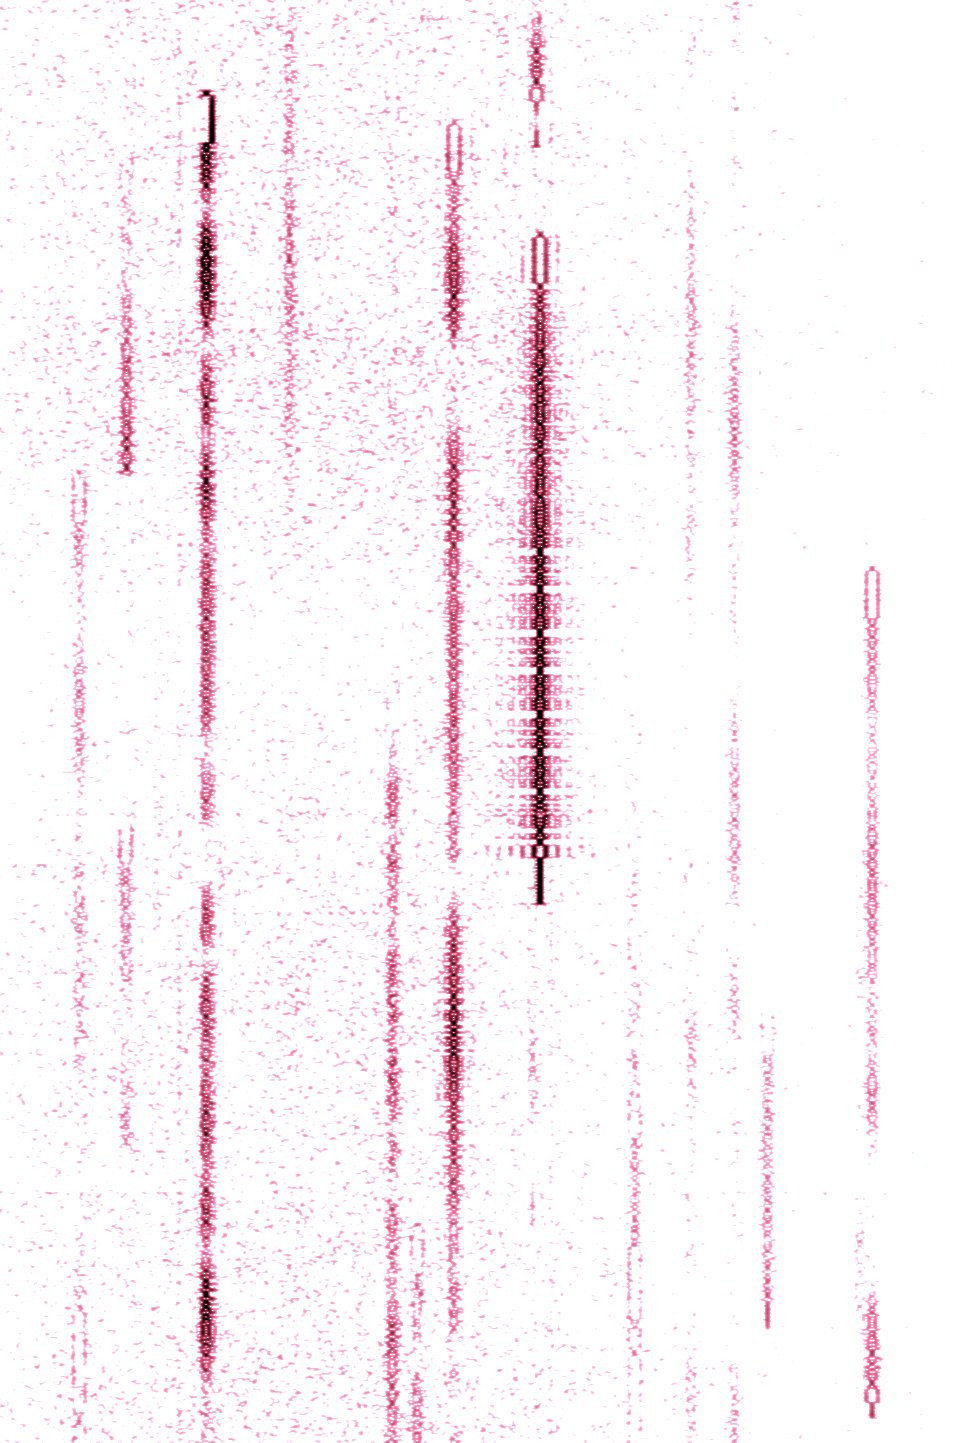
\includegraphics[width=.8\textwidth]{../pictures/matrix-inverted.jpg}
\caption*{\href{https://commons.wikimedia.org/wiki/File:PSK\_matrix.jpg}{Multiple PSK31 transmissions on the 20m digital modes band at around 14.07 MHz}.  Based on a public domain image by User:Mysid}
\end{figure}
